\chapter{GRAPHS}


\section{Introduction}
A \eax{graph} is a pair $G = (V,E)$, where $V$ is a set whose elements are called \eax{vertices} and $E \subseteq V \times V$ is a set of unordered pairs $\{v_{1},v_{2}\}$ of vertices, whose elements are called edges. Here, $(v_{1},v_{2})$ and $(v_{2},v_{1})$ are undistinguishable, and are simply denoted by $\{v_{1},v_{2}\}$ or $v_{1}v_{2}$.
\begin{figure}[h]
    \centering
    \begin{tikzpicture}[scale=1,
        every node/.style={circle, draw=\subjectcolor!80!black, fill=\subjectcolor!40!white, inner sep=2pt}]
        % Vertices
        \node (A) at (0, 0.2) {A};
        \node (B) at (2.1, -0.1) {B};
        \node (C) at (1.2, 1.6) {C};
        \node (D) at (3.1, 1.4) {D};
        \node (E) at (4.2, 0.1) {E};

        % Edges
        \draw (A) -- (B);
        \draw (B) -- (C);
        \draw (C) -- (A);
        \draw (B) -- (D);
        \draw (D) -- (E);
    \end{tikzpicture}
\end{figure}

The above shows a simple undirected graph on five vertices $V=\{A,B,C,D,E\}$ with edges $E=\{AB,AC,BC,BD,DE\}$. Here, simple and undirected are also terms to be defined in the context of graph theory.

\begin{definition}
    A graph is called a \eax{simple graph} if it has no loops (edges connecting a vertex to itself) and no multiple edges (more than one edge connecting the same pair of vertices). Otherwise, it is termed a \eax{multigraph}. A graph is called an \eax{undirected graph} if its edges have no orientation; that is, the edge $uv$ is identical to the edge $vu$. Otherwise, it is termed a \eax{directed graph}.
\end{definition}

In directed graphs, or \eax{digraph}s, one deals with $G = (V,E,s,t)$, where $s:E \to V$ gives the \eax{source node} of an edge and $t:E \to V$ gives the \eax{target node} of an edge. In this edge set $E$, $uv \neq vu$, unlike the case of a simple graph.

Structure-preserving maps are useful in graph theory too.

\begin{definition}
    Suppose we have two graphs $G = (V(G),E(G))$ and $H = (V(H),E(H))$. A function $f:V(G) \to V(H)$ is said to be a \eax{graph homomorphism} if $f$ preserves adjacency; that is, if $v_{1}v_{2} \in E(G)$, then $f(v_{1})f(v_{2}) \in E(H)$. If $f$ is also bijective and $f$ and $f^{-1}$ are both graph homomorphisms, then $f$ is termed a \eax{graph isomorphism}.
\end{definition}

We also term the group $\Aut(G)$ as the group of all graph isomorphisms of $G$, with the group operation of composition.

\begin{definition}
    Suppose we have two digraphs $G_{1} = (V_{1},E_{1},s_{1},t_{1})$ and $G_{2} = (V_{2},E_{2},s_{2},t_{2})$. A \eax{digraph homomorphism} is two maps $f_{V}:V_{1} \to V_{2}$ and $f_{E}:E_{1} \to E_{2}$ such that
    \begin{align}
        s_{2}(f_{E}(e)) = f_{V}(s_{1}(e)) \quad \text{ and } \quad t_{2}(f_{E}(e)) = f_{V}(t_{1}(e)).
    \end{align}
    That is, the source node of every image edge is the image node of every source node, and the target node of every image edge is the image node of every target node.
\end{definition}

One also discusses the neighbours of nodes.

\begin{definition}
    The \eax{degree of a node}, or the \eax{valency of a node}, is simply defined as the number of edges incident with the vertex. If $v$ is such a node in a graph $(V,E)$, then $\deg(v) = \#\{u \in V \mid vu \in E\}$. In digraphs, one defines the \eax{out-degree of a node} $v$ as the number of edges with $v$ as the source node, and the \eax{in-degree of a node} $v$ as the number of edges with $v$ as the target node.
\end{definition}

A \eax{regular graph} is one where every vertex has the same degree. We now discuss the first ever theorem (historically) in graph theory.

\begin{theorem}
    A finite (simple) graph $G$ has an even number of vertices of odd degree.
\end{theorem}

\begin{proof}
    Let $G = (V,E)$ be a graph. One can deduce that
    \begin{align}
        2 \cdot \# E(G) = \sum_{v \in V(G)} \deg(v).
    \end{align}
    Thus, there must be an even number of vertices of odd degree to keep the term on the left even.
\end{proof}


\section{Walks, Paths, and Cycles}

\begin{definition}
    A \eax{walk on a graph} $G$ is an alternating sequence of vertices and edges 
    \begin{align}
        (v_{0},e_{1},v_{1},e_{2},v_{2},\ldots,e_{k},v_{k})
    \end{align}
    such that for all $i$, $e_{i}$ is an edge between $v_{i-1}$ and $v_{i}$. The \eax{length of a walk}, in this case, is termed $k$.
\end{definition}


\begin{definition}
    If the edges $e_{1},e_{2},\ldots,e_{k}$ are distinct, then the walk is called a \eax{path on a graph}. A \eax{simple path} is one where the vertices $v_{0},v_{1},\ldots,v_{k}$ are also all distinct. Finally, a \eax{simple closed path}, or a \eax{cycle on a graph}, is one where $v_{0} = v_{k}$ and the rest are distinct.
\end{definition}

A \eax{metric on a graph} between two vertices $d(v_{1},v_{2})$ is defined as the length of the shortest walk between $v_{1}$ and $v_{2}$. This walk is always a path since if it's not, there is a repetition of edges, and appropriate middle edges and vertices can be deleted to form a path or a shorter walk. If no such path exists, then $d(v_{1},v_{2}) = \infty$. Thus, a finite \eax{connected graph} $G$ is one where $d(v_{1},v_{2}) < \infty$ for all $v_{1},v_{2} \in V(G)$.\\ \\
\textit{August 21st.}

\subsection{The K\"onigsberg Bridge Problem}

The following figure illustrates the famous problem of the \eax{K\"onigsberg bridge problem}.

\begin{figure}[h]
    \centering
    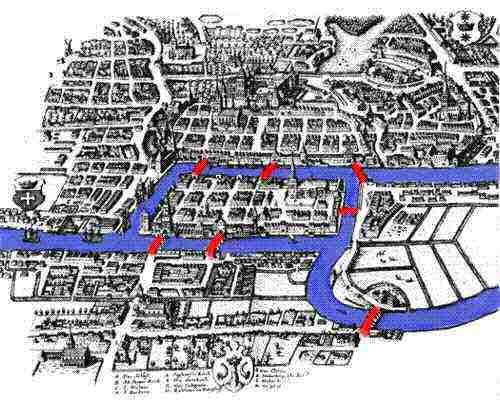
\includegraphics[width=0.3\textwidth]{chapters/konigsberg.jpg}
    \caption{The Seven Bridges of K\"onigsberg}
    \label{fig:konigsberg}
\end{figure}

Euler asked the question if one could cross each of the seven bridges exactly once and come back to the same side of the riverbank; this is formally considered as the first ever problem in graph theory.

Here, an \eax{Eulerian circuit} is defined, which is a closed path using every edge in the graph exactly once. A graph with an Eulerian circuit is termed an \eax{Eulerian graph}.

\begin{figure}[h]
    \centering
    \begin{tikzpicture}[scale=1.2,
        every node/.style={circle, draw=\subjectcolor!80!black, fill=\subjectcolor!40!white, inner sep=2pt}]
        
        % Nodes
        \node (A) at (0, 1.5) {A}; % North bank
        \node (B) at (0, 0) {B};   % South bank
        \node (C) at (2, 0.75) {C}; % Island (Kneiphof)
        \node (D) at (4, 0.75) {D}; % East bank or another land mass

        % Edges (bridges)
        \draw (A) -- (B);         % Bridge 1
        \draw (A) -- (C);         % Bridge 2
        \draw (A) -- (C);         % Bridge 3 (double line)
        \draw (B) -- (C);         % Bridge 4
        \draw (B) -- (C);         % Bridge 5 (double line)
        \draw (A) -- (D);         % Bridge 6
        \draw (C) -- (D);         % Bridge 7

    \end{tikzpicture}
    \caption{Graph Representation of the Seven Bridges of K\"onigsberg}
    \label{fig:konigsberg_graph}
\end{figure}
(Above graph to be fixed.)

\begin{theorem}
    A finite multigraph $G$ is Eulerian if and only if $G$ is connected and is a edge-disjoint union of cycle $G = C_{1} \cup C_{2} \cup \cdots \cup C_{m}$ where $C_{i}$'s are cycles with no common edges.
\end{theorem}

\begin{proof}
    Suppose $G = C_{1} \cup C_{2} \cup \cdots \cup C_{m}$ where $C_{i}$'s are edge-disjoint cycles. For $m = 2$, choose $v \in V(C_{1}) \cap V(C_{2})$; such a $v$ must exist or else the graph is disconnected. Starting at $v$, exhaust all edges in $C_{1}$ using the trivial Eulerian circuit and return to $v$. Do the same with $C_{2}$, and you have found the Eulerian circuit. Now apply the induction hypothesis; for an arbitrary $m$, choose $v \in V(C_{1} \cup C_{2} \cup \cdots \cup C_{m-1}) \cap V(C_{m})$. Again, such a $v$ must exist since $G$ is connected. Starting at $v$, exhaust all edges in $C_{1}$ using the trivial Eulerian circuit and return to $v$, then use the Eulerian circuit in $C_{1} \cup C_{2} \cup \cdots \cup C_{m-1}$ formed via the induction hypothesis.

    For the converse, an Eulerian circuit on the graph involves all edges and returns to the same vertex, so $G$ must be connected. To show the disjoint union of cycles, find a cycle in the Eulerian circuit; there must exist at least one since, if not, the circuit itself is a cycle. Delete the edges from this cycle, and join the starting vertex and ending vertex in of this cycle in the circuit. Repeat the same until the resulting Eulerian circuit is a cycle. The disjoint union of this cycle and the cycles removed is the starting circuit.
\end{proof}

One can show a better result.

\begin{theorem}
    A finite multigraph $G$ is Eulerian if and only if $G$ is connected and every vertex has an even degree.
\end{theorem}

\begin{proof}
    If $G$ is Eulerian, then $G$ is connected by the previous theorem, and $G = C_{1} \cup C_{2} \cup \cdots \cup C_{m}$, a union of disjoint cycles. Also, for $v \in V(G)$,
    \begin{align}
        \deg_{G}(v) = \sum_{i=1}^{m} \deg_{C_{i}}(v) = 2 \left( \sum_{i=1}^{m} \1_{\{v \in C_{i}\}} \right).
    \end{align}
    Thus, $\deg_{G}(v)$ is even for all $v \in V(G)$.

    For the converse implication, assume $G$ is connected and every vertex has an even degree. We will show that $G$ is Eulerian. Start by choosing any cycle $C_{1}$ in $G$. Remove the edges of $C_{1}$ from $G$ to form a subgraph $G'$. Since every vertex in $G$ has even degree, removing the edges of $C_{1}$ leaves every vertex in $G'$ with even degree. If $G'$ is connected, repeat the process to find another cycle $C_{2}$ in $G'$. Continue this process until no edges remain. If $G'$ is disconnected at any step, then each connected component of $G'$ must also have all vertices of even degree. By the same argument, we can find cycles in each connected component and remove their edges. Eventually, all edges of $G$ are partitioned into disjoint cycles. Since $G$ is connected, these cycles can be combined into a single Eulerian circuit by appropriately traversing edges between cycles. Thus, $G$ is Eulerian.
\end{proof}

\section{Adjacency}

For a simple graph $G = (V,E)$, an \eax{adjacency matrix} can be defined of dimension $\# V \times \# V$, with $a_{v,w} = 1$ if $vw \in E$, and $a_{v,w} = 0$ otherwise. For a multigraph, $a_{v,w}$ is the number of edges between vertices $v$ and $w$. Similarly, for a directed graph, $a_{v,w} = 1$ if $vw \in E$ and $a_{w,v} = 0$ otherwise. For an undirected graph, the adjacency matrix $A$ is symmetric and consists of only 1's and 0's. 

\begin{figure}[h]
    \centering
    \begin{tikzpicture}[scale=1.2,
        every node/.style={circle, draw=\subjectcolor!80!black, fill=\subjectcolor!40!white, inner sep=2pt}]
        
        % Nodes with slight deviations
        \node (A) at (0.1, 1.6) {$v_{1}$};
        \node (B) at (1.6, 1.4) {$v_{2}$};
        \node (C) at (-0.1, -0.1) {$v_{3}$};
        \node (D) at (1.4, 0.1) {$v_{4}$};

        % Edges
        \draw (A) -- (B);
        \draw (A) -- (C);
        \draw (B) -- (D);
        \draw (C) -- (D);
        \draw (B) -- (C);

    \end{tikzpicture}
    \caption{A simple graph with four vertices}
    \label{fig:graph_example}
\end{figure}
The adjacency matrix for the graph in Figure~\ref{fig:graph_example} is given as
$
A =
\begin{bmatrix}
0 & 1 & 1 & 0 \\
1 & 0 & 1 & 1 \\
1 & 1 & 0 & 1 \\
0 & 1 & 1 & 0
\end{bmatrix}
$. For two graphs $G_{1}$ and $G_{2}$ to be isomorphic, one can show that $A(G_{1})$ must be similar to $A(G_{2})$. Moreover, to count the number of walks from $v$ to $w$ of length $k$, one can use the $k$-th power of the adjacency matrix: the entry $(i,j)$ of $A^{k}$ gives the number of walks of length $k$ from vertex $v_{i}$ to vertex $v_{j}$.